%! Author = Juniell
%! Date = 06.05.2021

% Preamble
\documentclass[a4paper, 14pt]{extarticle}

% Packages
\usepackage[T2A]{fontenc}
\usepackage{natbib}
\usepackage{graphicx}
\usepackage[english, russian]{babel}
\usepackage{fontspec}
\usepackage{amsmath}
\usepackage{amsfonts}
\usepackage{amssymb}
\usepackage{amsthm}
\usepackage{mathtools}
\usepackage{mathrsfs}
\usepackage{fullpage}
\usepackage{ulem}
\usepackage{setspace}
\usepackage{listings}
\usepackage{indentfirst}
\usepackage[left=2cm,right=1.5cm,top=2cm,bottom=2cm]{geometry}
\usepackage{xcolor}
\usepackage{float}
\usepackage{csquotes}
\usepackage{hyperref}
\usepackage{graphics}

\definecolor{urlcolor}{HTML}{0000FF} % цвет ссылок
\definecolor{linkcolor}{HTML}{000000} % цвет гиперссылок
\hypersetup{pdfstartview=FitH, linkcolor=linkcolor, urlcolor=urlcolor, colorlinks=true}

\setmainfont{Times New Roman}
\setlength{\parindent}{5ex}
\setlength{\parskip}{1em}
\renewcommand{\baselinestretch}{1}

\graphicspath{{resources/Images}}

\definecolor{buzzlightyear}{HTML}{8757A5}
\definecolor{grass}{HTML}{738D06}
\definecolor{literal}{HTML}{F18A2B}
\definecolor{commentcolor}{HTML}{8E908B}

\lstdefinestyle{habrstyle}{
    backgroundcolor=\color{white},
    commentstyle=\color{commentcolor},
    keywordstyle=\bfseries\color{buzzlightyear},
    numberstyle=\tiny\color{commentcolor},
    stringstyle=\color{grass},
    basicstyle=\ttfamily\footnotesize,
    breakatwhitespace=false,
    breaklines=true,
    captionpos=b,
    keepspaces=true,
    numbers=left,
    numbersep=5pt,
    showspaces=false,
    showstringspaces=false,
    showtabs=false,
    tabsize=4,
    language=Python
}

\lstset{style=habrstyle}


% Document
\begin{document}
% Титульный лист
    \begin{center}
        \begin{center}
            \hfill \break
            \normalsize{Санкт-Петербургский государственный политехнический}\\
            \normalsize{университет Петра Великого}\\
            \hfill \break
            \normalsize{\textbf{Высшая школа интеллектуальных систем и}}\\
            \normalsize{\textbf{суперкомпьютерных технологий}}\\
            \hfill \break
            \hfill \break
            \hfill \break
            \hfill \break
            \hfill \break
            \normalsize{Отчёт по лабораторной работе №3}\\
            \normalsize{Дисциплина: Телекоммуникационные технологии}\\
            \normalsize{Тема: Апериодические сигналы}\\
        \end{center}
        \hfill \break
        \hfill \break
        \hfill \break
        \hfill \break
        \hfill \break
        \hfill \break
        \hfill \break
        \hfill \break
        \hfill \break
        \hfill \break
        \begin{tabbing}
            Выполнил студент гр. 3530901/80201 \`В.А. Пучкина\\
            \\
            Преподаватель: \`Н.В. Богач\\
        \end{tabbing}
        \hfill \break
        \hfill \break
        \hfill \break
        \hfill \break
        \begin{center}
            Санкт-Петербург\\
            2021
        \end{center}
        \thispagestyle{empty}
    \end{center}

% Оглавление
    \newpage
    \tableofcontents

% Список иллюстраций
    \newpage
    \listoffigures

% Список листингов
    \newpage
    \lstlistoflistings

% ---------------------------------------------- Упражнение 3.1 ----------------------------------------------
    \newpage
    \section{Упражнение 3.1}
    \label{sec:task1}

    В этому упражнении необходимо загрузить файл \texttt{chap03.ipynb}, изучить его, просмотреть пояснения и запустить примеры.
    Кроме того, в примере с утечкой предлагается заменить окно Хэмминга на любое другое, предоставляемое NumPy.

    Итак, изучим примеры.

    \begin{figure}[H]
        \centering
        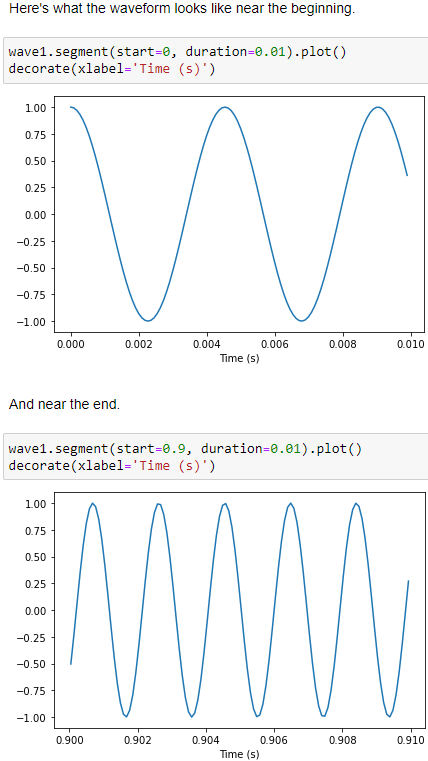
\includegraphics[width=0.6\linewidth]{resources/Images/task1_check_chirp}
        \caption{Изучение и проверка примеров (Chirp).}
        \label{fig:task1_check_chirp}
    \end{figure}

    \begin{figure}[H]
        \centering
        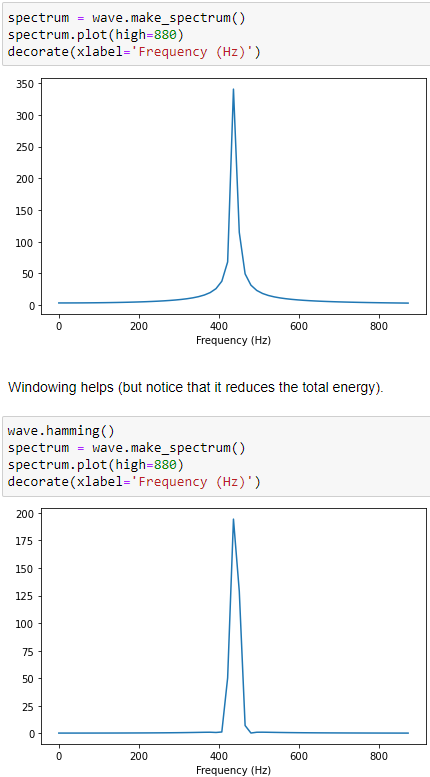
\includegraphics[width=0.75\linewidth]{resources/Images/task1_check_leakage}
        \caption{Изучение и проверка примеров (Влияние использования окон на утечку).}
        \label{fig:task1_check_leakage}
    \end{figure}

    \begin{figure}[H]
        \centering
        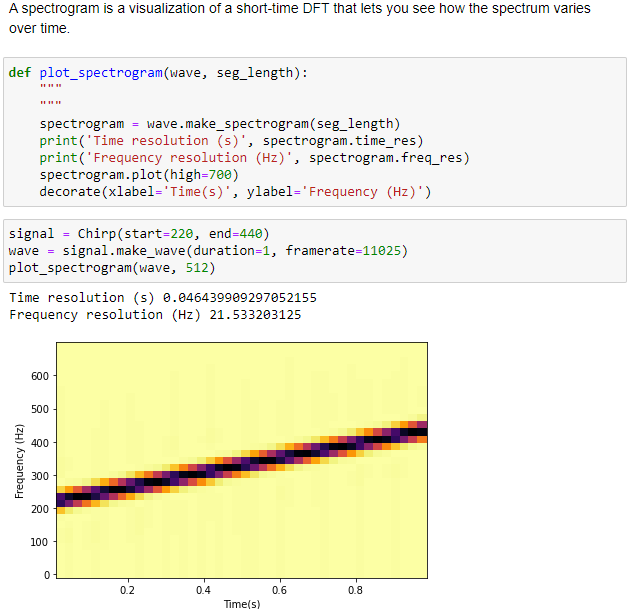
\includegraphics[width=0.75\linewidth]{resources/Images/task1_check_spectrogram}
        \caption{Изучение и проверка примеров (Спектрограмма).}
        \label{fig:task1_check_spectrogram}
    \end{figure}

    Все примеры были изучены и запущены. Теперь попробуем использовать другие окна в примере с Хэммингом.
    Для этого сначала создадим аналогичный сигнал, получим его \texttt{wave} и вычислим спектр с использованием окна Бартлетта.

    \begin{lstlisting}[caption= Создание сигнала и получение спектра с использованием \texttt{bartlett}., label={lst:task1_leakage_bartlett}]
signal = SinSignal(freq=440)
wave = signal.make_wave(signal.period * 30.25)

wave.window(numpy.bartlett(len(wave)))
spectrum = wave.make_spectrum()
spectrum.plot(high=880)
decorate(xlabel='Frequency (Hz)')
    \end{lstlisting}

    Теперь получим спектр, используя окно Блэкмана.

    \begin{lstlisting}[caption= Получение спектра с использованием \texttt{blackman}., label={lst:task1_leakage_blackman}]
wave.window(numpy.blackman(len(wave)))
spectrum = wave.make_spectrum()
spectrum.plot(high=880)
decorate(xlabel='Frequency (Hz)')
    \end{lstlisting}

    \begin{figure}[H]
        \centering
        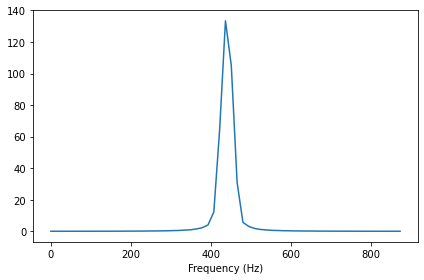
\includegraphics[width=0.8\linewidth]{resources/Images/task1_leakage_bartlett}
        \caption{Спектр, полученный с помощью окна bartlett.}
        \label{fig:task1_leakage_bartlett}
    \end{figure}

    \begin{figure}[H]
        \centering
        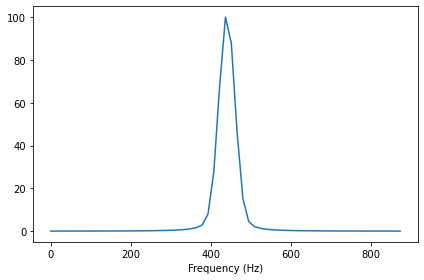
\includegraphics[width=0.8\linewidth]{resources/Images/task1_leakage_blackman}
        \caption{Спектр, полученный с помощью окна blackman.}
        \label{fig:task1_leakage_blackman}
    \end{figure}

    Если сравнить полученные спектры со спектром, полученным без использования оконных функций
    (Рис.\ref{fig:task1_check_leakage}, верхний график), можно заметить, что утечки действительно уменьшились.
    Однако, при сравнении этих результатов с результатом после использования окна Хэмминга (Рис.\ref{fig:task1_check_leakage}, нижний график)
    видно, что общая энергия становится ещё ниже. Это связано с тем, что окно Хэмминга - это окно-<<вездеход>>, а вот
    окна Бартлетта и Блэкмана являются оптимальными для некоторых случаев.

    В ходе выполнения данного упражнения были получены знания работе с \texttt{Chirp}, утечками и оконными функциями.
    Также были рассмотрены спектрограммы и их возможности.
    Кроме того, были сравнены результаты применения различных оконных функций для получения спектра.
    Был сделан вывод, что окна Бартлетта и Блэкмана оптимальны в некоторых случаях, а окно Хэмминга является универсальным.

    \newpage

% ---------------------------------------------- Упражнение 3.2 ----------------------------------------------
    \section{Упражнение 3.2}
    \label{sec:task2}

    Во втором упражнении необходимо написать класс \texttt{SawtoothChirp}, расширяющий \texttt{Chirp} и переопределяющий
    \texttt{evaluate} для генерации пилообразного сигнала с линейно увеличивающейся (или уменьшающейся) частотой.

    Итак, начнём с написания класса \texttt{SawtoothChirp}.

    \begin{lstlisting}[caption= Создание класса \texttt{SawtoothChirp}., label={lst:task2_create_class}]
PI2 = numpy.pi * 2

class SawtoothChirp(Chirp):
    def evaluate(self, ts):
        freqs = numpy.linspace(self.start, self.end, len(ts))
        dts = numpy.diff(ts, prepend=0)
        dphis = PI2 * freqs * dts
        phases = numpy.cumsum(dphis)
        cycles = phases / PI2
        # From SawtoothSignal
        frac, _ = numpy.modf(cycles)
        ys = normalize(unbias(frac), self.amp)
        return ys
    \end{lstlisting}

    Данный класс расширяет класс \texttt{Chirp} и переопределяет его метод \texttt{evaluate}.

    Теперь проверим работу нашего класса, создав пилообразный \texttt{chirp}.
    Затем преобразуем его к \texttt{wave} и получим аудио.

    \begin{lstlisting}[caption= Создание и работа с сигналом., label={lst:task2_work_with_chirp}]
sawtooth_signal = SawtoothChirp(start=900, end=350)
sawtooth_wave = sawtooth_signal.make_wave(duration=1, framerate=4000)
sawtooth_wave.apodize()
sawtooth_wave.make_audio()
    \end{lstlisting}

    Звук очень необычный и похож на включенный задом наперёд звук сирены. Теперь построим спектрограмму нашего сигнала.

    \begin{lstlisting}[caption= Создание и вывод спектрограммы., label={lst:task2_chirp_spectrogram}]
spectrogram = sawtooth_wave.make_spectrogram(200)
spectrogram.plot()
decorate(xlabel='Time (s)', ylabel='Frequency (Hz)')
    \end{lstlisting}

    На полученной спектрограмме хорошо видно, как гармоники с наложенными частотами отражаются от частоты заворота.
    Именно так на спектрограмме можно увидеть эффект биений. Кроме того, если вслушаться в полученный звук, то биения можно
    услышать как фоновое шипение.

    \begin{figure}[h]
        \centering
        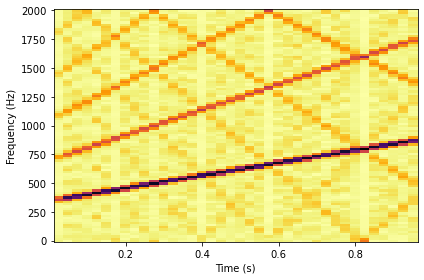
\includegraphics[width=0.8\linewidth]{resources/Images/task2_spectrogram}
        \caption{Спектрограмма полученного сигнала.}
        \label{fig:task2_chirp_spectrogram}
    \end{figure}

    В ходе выполнения данного задания был описан класс \texttt{SawtoothChirp}, генерирующий пилообразный сигнал с линейно
    увеличивающейся (или уменьшающейся) частотой. С помощью этого класса был создан сигнал, после чего была получена его
    спектрограмма. На спектрограмме хорошо виден эффект биений.

    \newpage

% ---------------------------------------------- Упражнение 3.3 ----------------------------------------------
    \section{Упражнение 3.3}
    \label{sec:task3}

    В третьем упражнении необходимо создать пилообразный \texttt{chirp} с частотой, меняющейся от 2500 до 3000 Гц.
    Затем на основе этого сигнала сгенерировать сигнал длительностью 1 с и частотой кадров 20 кГц. После этого необходимо
    предположить, каким будет его спектр, и сравнить предположения с самим спектром.

    Итак, создадим пилообразный \texttt{chirp} с требуемой частотой и сгенерируем сигнал длительностью 1 с и частотой кадров 20 кГц.
    Тут же прослушаем его.

    \begin{lstlisting}[caption= {Создание сигнала, получение \texttt{wave} и аудио.}, label={lst:task3_wave_audio}]
sawtooth_signal = SawtoothChirp(start=2500, end=3000)
sawtooth_wave = sawtooth_signal.make_wave(duration=1, framerate=20000)
sawtooth_wave.make_audio()
    \end{lstlisting}

    Звук этого сигнала сильно режет слух и кажется слишком резким и пищащим.

    Предположим, какой спектр будет иметь этот сигнал. Так как частота изменяется от 2500 до 3000 Гц, то в этом диапазоне
    ожидается увидеть всплеск. Кроме того, мы помним, что пилообразный сигнал имеет и чётные, и нечётные гармоники.
    Первая гармоника ожидается в диапазоне от 5000 до 6000 Гц, однако она должна быть поменьше предыдущего всплеска.
    Вторая гармоника тогда должна быть ещё меньше находиться в диапазоне от 7500 до 9000 Гц. Следующие гармоники
    накладываются друг на друга, а потому на всех остальных частотах должны быть небольшие колебания.

    Теперь, наконец, получим спектр нашего сигнала и сравним его с ожидаемым спектром.

    \begin{lstlisting}[caption= Создание и вывод спектра., label={lst:task3_spectrum}]
sawtooth_wave.make_spectrum().plot()
decorate(xlabel='Frequency (Hz)')
    \end{lstlisting}

    Как видно из Рис.\ref{fig:task3_spectrum} наши ожидания совпали с реальным спектром.

    \begin{figure}[H]
        \centering
        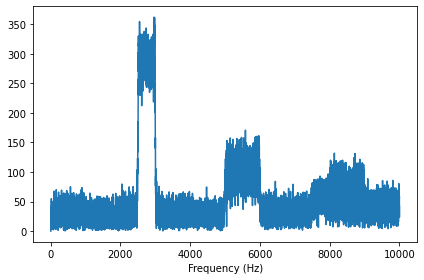
\includegraphics[width=0.8\linewidth]{resources/Images/task3_spectrum}
        \caption{Спектр полученного сигнала.}
        \label{fig:task3_spectrum}
    \end{figure}

    В ходе выполнения данного упражнения был создан пилообразный \texttt{chirp} с частотой, меняющейся от 2500 до 3000 Гц.
    После этого был сгенерированы его аудио и \texttt{wave}. Полученный сигнал режет слух и кажется очень неприятным и пищащим.
    Далее было сделано предположение о том, как будет выглядеть его спектр. После чего был получен спектр и сравнён с ожиданиями.
    Наше ожидания совпали с самим спектром.

    \newpage

% ---------------------------------------------- Упражнение 3.4 ----------------------------------------------
    \section{Упражнение 3.4}
    \label{sec:task4}

    В этом упражнении происходит работа с глиссандо.
    Глиссандо - это нота, меняющаяся от одной высоты до другой, т.е. своеобразный \texttt{chirp}.
    Необходимо найти звук глиссандо и изучить спектрограмму его нескольких секунд.

    Итак, была выбрана \href{https://freesound.org/people/InspectorJ/sounds/411728/}{эта} запись глиссандо скрипки.
    Теперь считаем файл и выведем аудио.

    \begin{lstlisting}[caption= Считывание и воспроизведение файла., label={lst:task4_wave}]
wave = read_wave('resources/Sounds/task4_violin_glissando.wav')
wave.make_audio()
    \end{lstlisting}

    Теперь выделим небольшой сегмент и получим его аудио.

    \begin{lstlisting}[caption= Работа с сегментом., label={lst:task4_segment}]
segment = wave.segment(start=0.17, duration=1)
segment.make_audio()
    \end{lstlisting}

    И наконец, получим спектрограмму этого сегмента.

    \begin{lstlisting}[caption= Получение спекограммы., label={lst:task4_segment_spectrogram}]
segment.make_spectrogram().plot()
decorate(xlabel='Time (s)', ylabel='Frequency (Hz)')
    \end{lstlisting}

    \begin{figure}[h]
        \centering
        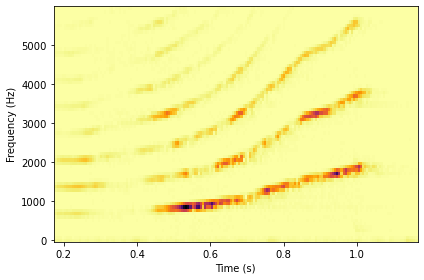
\includegraphics[width=0.8\linewidth]{resources/Images/task4_segment_spectrogram}
        \caption{Спектрограмма звука глиссандо.}
        \label{fig:task4_segment_spectrogram}
    \end{figure}

    Полученная спектрограмма выглядит очень интересно, на ней хорошо заметно глиссандо.

    В ходе выполнения данного упражнения была получена спектрограмма глиссандо скрипки.

    \newpage

% ---------------------------------------------- Упражнение 3.5 ----------------------------------------------
    \section{Упражнение 3.5}
    \label{sec:task5}

    В этом упражнении необходимо написать класс \texttt{TromboneGliss}, расширяющий \texttt{Chirp} и переопределяющий
    \texttt{evaluate}. Затем необходимо создать сигнал, имитирующий глиссандо на тромбоне от C3 (262 Гц) до F3 (349 Гц)
    и обратно до C3. После этого нужно изучить спектрограмму полученного сигнала.

    Итак, сначала напишем класс \texttt{TromboneGliss}.

    \begin{lstlisting}[caption= Класс \texttt{TromboneGliss}., label={lst:task5_class}]
class TromboneGliss(Chirp):
     def evaluate(self, ts):
        l1, l2 = 1.0 / self.start, 1.0 / self.end
        lengths = numpy.linspace(l1, l2, len(ts))
        freqs = 1 / lengths
        dts = numpy.diff(ts, prepend=0)
        dphis = PI2 * freqs * dts
        phases = numpy.cumsum(dphis)
        ys = self.amp * numpy.cos(phases)
        return ys
    \end{lstlisting}

    Этот класс расширяет \texttt{Chirp} и переопределяет \texttt{evaluate}. Теперь создадим первую половину сигнала:
    глиссандо от C3 (262 Гц) до F3 (349 Гц). Тут же прослушаем его.

    \begin{lstlisting}[caption= Создание сигнала глиссандо от C3 до F3., label={lst:task5_signal_up}]
signal_up = TromboneGliss(262, 349)
wave_up = signal_up.make_wave(duration=1)
wave_up.make_audio()
    \end{lstlisting}

    Полученный звук действительно напоминает глиссандо. Теперь создадим сигнал глиссандо от F3 до C3 и прослушаем его.

    \begin{lstlisting}[caption= Создание сигнала глиссандо от F3 до C3., label={lst:task5_signal_down}]
signal_down = TromboneGliss(349, 262)
wave_down = signal_down.make_wave(duration=1)
wave_down.make_audio()
    \end{lstlisting}

    Осталось только склеить оба этих сигнала, вывести спектрограмму и прослушать результат.

    \begin{lstlisting}[caption= Создание итогового сигнала и получение его спектрограммы., label={lst:task5_signal_result}]
wave_up_down = wave_up | wave_down
spectrogram = wave_up_down.make_spectrogram(1024)
spectrogram.plot(high=1000)
decorate(xlabel='Time (s)', ylabel='Frequency (Hz)')
wave_up_down.make_audio()
    \end{lstlisting}

    \begin{figure}[h]
        \centering
        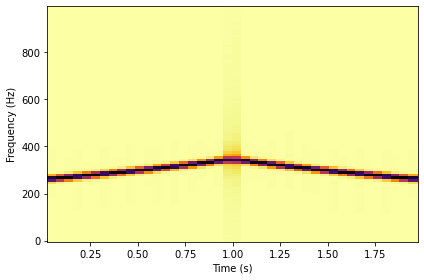
\includegraphics[width=0.8\linewidth]{resources/Images/task5_spectrogram}
        \caption{Спектрограмма итогового сигнала.}
        \label{fig:task5_spectrogram}
    \end{figure}

    Как видно из спектрограммы (Рис.\ref{fig:task5_spectrogram}), полученный сигнал больше похож на линейный \texttt{chirp}.
    Его же звук действительно напоминает глиссандо от C3 до F3 и обратно в C3.

    В ходе выполнения данного упражнения был написан класс \texttt{TromboneGliss}, генерирующий сигнал глиссандо на тромбоне.
    С помощью этого класса был создан сигнал, имитирующий глиссандо на тромбоне от C3 до F3 и обратно до C3.
    У этого сигнала была получена спектрограмма, изучив которую, был сделан вывод, что этот сигнал больше похож на
    линейный \texttt{chirp}.

    \newpage

% ---------------------------------------------- Упражнение 3.6 ----------------------------------------------
    \section{Упражнение 3.6}
    \label{sec:task6}

    В этом упражнении необходимо найти запись серии гласных звуков и посмотреть на их спектрограмму. Эксперимент
    заключается в попытке определения различных гласных звуков на спектрограмме.

    Был выбран первый отрывок гласных из \href{https://freesound.org/people/cbelloso/sounds/523055/}{этой} записи.
    На этом отрывке ребёнок произносит звуки <<А>>, <<Э>>, <<И>>, <<О>> и <<У>>. Теперь считаем файл, получим необходимый сегмент, прослушаем его и вывеем спектрограмму.

    \begin{lstlisting}[caption= Формирование нужного сгемента и вывод спектрограммы., label={lst:task5_signal_down}]
w = read_wave('resources/Sounds/task6_vowels.wav')
wave = w.segment(start=0, duration=4.4)
wave.make_spectrogram(1024).plot(high=1000)
decorate(xlabel='Time (s)', ylabel='Frequency (Hz)')
wave.make_audio()
    \end{lstlisting}

    \begin{figure}[h]
        \centering
        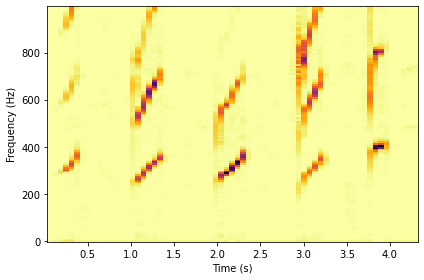
\includegraphics[width=0.65\linewidth]{resources/Images/task6_spectrogram}
        \caption{Спектрограмма серии гласных звуков.}
        \label{fig:task6_spectrogram}
    \end{figure}

    Итак, мы получили спектрограмму гласных звуков. Догадаться, какой именно звук представлен на спектрограмме,
    я могу только по порядку. Также из спектрограммы видно, что звук <<И>> имеет самую малую частоту, остальные же звуки
    на спектрограмме  очень похожи.

    Теперь получим сегмент со звуком <<А>> и изучим его спектр.

    \begin{lstlisting}[caption= Вывод спектра звука <<А>>., label={lst:task5_segment_a}]
segment_a = wave.segment(start=0.25, duration=0.7)
segment_a.make_spectrum().plot(high=1000)
segment_a.make_audio()
    \end{lstlisting}

    \begin{figure}[H]
        \centering
        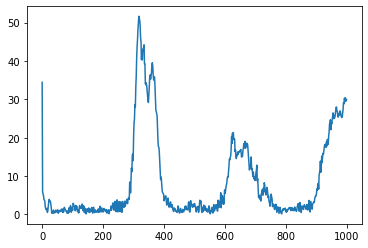
\includegraphics[width=0.7\linewidth]{resources/Images/task6_spectrum_a}
        \caption{Спектр звука <<А>>.}
        \label{fig:task6_spectrogram}
    \end{figure}

    Из спектра видно, что самая высокоамплитудная частота находится примерно на 300 Гц.
    Теперь получим сегмент со звуком <<Э>> и изучим его спектр.

    \begin{lstlisting}[caption= Вывод спектра звука <<Э>>., label={lst:task5_segment_e}]
segment_e = wave.segment(start=0.85, duration=0.7)
segment_e.make_spectrum().plot(high=1000)
segment_e.make_audio()
    \end{lstlisting}

    \begin{figure}[H]
        \centering
        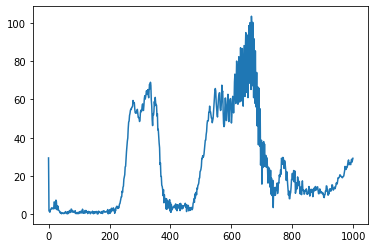
\includegraphics[width=0.7\linewidth]{resources/Images/task6_spectrum_e}
        \caption{Спектр звука <<Э>>.}
        \label{fig:task6_spectrum_e}
    \end{figure}

    Сегмент <<Э>> имеет самые высокие пики примерно на 700 и 350 Гц.
    Теперь получим сегмент со звуком <<И>> и изучим его спектр.

    \begin{lstlisting}[caption= Вывод спектра звука <<И>>., label={lst:task5_segment_i}]
segment_i = wave.segment(start=1.8, duration=0.7)
segment_i.make_spectrum().plot(high=1000)
segment_i.make_audio()
    \end{lstlisting}

    \begin{figure}[h]
        \centering
        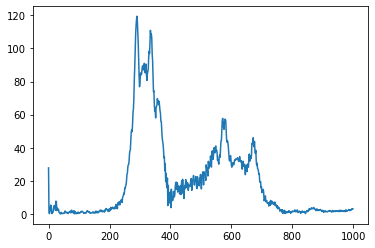
\includegraphics[width=0.7\linewidth]{resources/Images/task6_spectrum_i}
        \caption{Спектр звука <<И>>.}
        \label{fig:task6_spectrum_i}
    \end{figure}

    Сегмент <<И>> имеет высокие пики примерно на 300 и 600 Гц.
    Теперь получим сегмент со звуком <<О>> и изучим его спектр.

    \begin{lstlisting}[caption= Вывод спектра звука <<О>>., label={lst:task5_segment_o}]
segment_o = wave.segment(start=2.6, duration=0.7)
segment_o.make_spectrum().plot(high=1000)
segment_o.make_audio()
    \end{lstlisting}

    Сегмент <<О>> имеет высокий пик примерно на 750 Гц.
    Теперь получим сегмент со звуком <<У>> и изучим его спектр.

    \begin{lstlisting}[caption= Вывод спектра звука <<У>>., label={lst:task5_segment_u}]
segment_u = wave.segment(start=3.7, duration=0.5)
segment_u.make_spectrum().plot(high=1000)
segment_u.make_audio()
    \end{lstlisting}

    \begin{figure}[H]
        \centering
        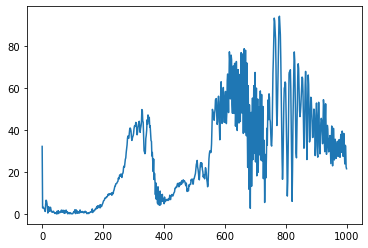
\includegraphics[width=0.7\linewidth]{resources/Images/task6_spectrum_o}
        \caption{Спектр звука <<О>>.}
        \label{fig:task6_spectrum_o}
    \end{figure}

    \begin{figure}[H]
        \centering
        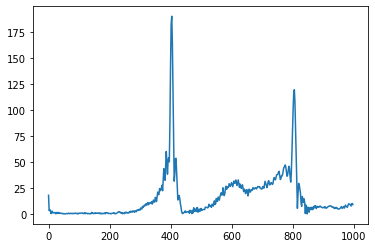
\includegraphics[width=0.7\linewidth]{resources/Images/task6_spectrum_u}
        \caption{Спектр звука <<У>>.}
        \label{fig:task6_spectrum_u}
    \end{figure}

    Сегмент <<У>> имеет самые высокие пики на 400 и 800 Гц.

    В ходе этого упражнения была найдена и проанализирована запись серии гласных звуков, а также изучена её спектрограмма.
    Кроме того, были изучены спектры отдельных гласных звуков.

    \newpage

% ---------------------------------------------- Упражнение 3.6 ----------------------------------------------
    \section{Выводы}
    \label{sec:conclusions}

    В ходе выполнения данной лабораторной работы были изучены спектры, спектрограммы, \texttt{chirp} и глиссандо.
    Был создан класс \texttt{SawtoothChrip}, генерирующий пилообразный сигнал с линейно увеличивающейся
    (или уменьшающейся) частотой, после чего этот класс был протестирован. Также был создан и протестирован класс
    \texttt{TromboneGliss}, генерирующий сигнал глиссандо на тромбоне. Кроме того, были изучены эффект утечек и
    оконные функции, сформирована и изучена спектрограмма гласных звуков и спектры отдельных звуков.


\end{document}